% v6.0 Marginal Component Contributions (Shapley Values)
% Replaces: tab:shapley-contributions in appendix_m
% Horizontal bar chart showing each model's marginal contribution

\begin{figure}[htbp]
\centering
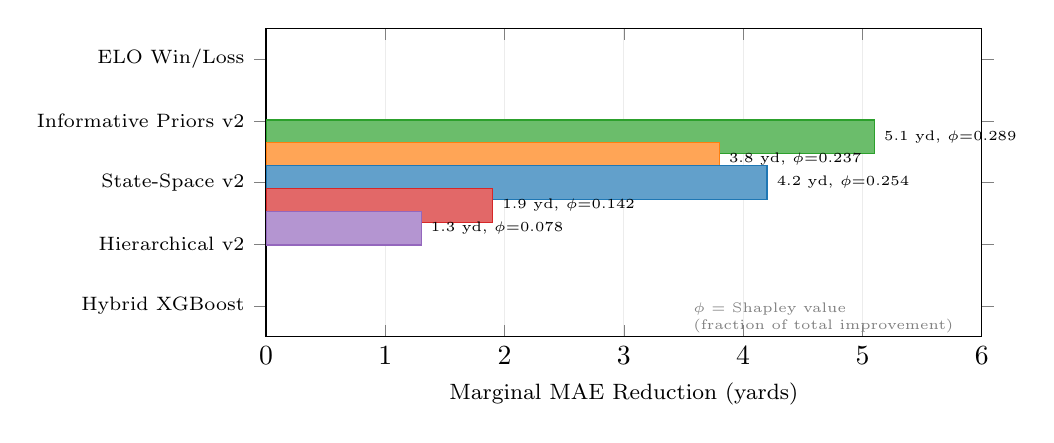
\begin{tikzpicture}
\definecolor{colSS}{RGB}{31,119,180}
\definecolor{colHier}{RGB}{255,127,14}
\definecolor{colXGB}{RGB}{44,160,44}
\definecolor{colIP}{RGB}{214,39,40}
\definecolor{colELO}{RGB}{148,103,189}

\begin{axis}[
  width=0.88\textwidth,
  height=5.5cm,
  xbar,
  bar width=12pt,
  xmin=0, xmax=6,
  xlabel={Marginal MAE Reduction (yards)},
  xlabel style={font=\footnotesize},
  ytick={1,2,3,4,5},
  yticklabels={
    {ELO Win/Loss},
    {Informative Priors v2},
    {State-Space v2},
    {Hierarchical v2},
    {Hybrid XGBoost}
  },
  yticklabel style={font=\scriptsize},
  y dir=reverse,
  grid=major,
  grid style={gray!15},
  xmajorgrids=true,
  ymajorgrids=false,
  enlarge y limits={abs=0.5},
  nodes near coords,
  nodes near coords style={font=\tiny, anchor=west},
  point meta=explicit symbolic,
]

% Bars colored by component
\addplot[fill=colXGB!70, draw=colXGB] coordinates {
  (5.1, 1) [{5.1 yd, $\phi$=0.289}]
};
\addplot[fill=colHier!70, draw=colHier] coordinates {
  (3.8, 2) [{3.8 yd, $\phi$=0.237}]
};
\addplot[fill=colSS!70, draw=colSS] coordinates {
  (4.2, 3) [{4.2 yd, $\phi$=0.254}]
};
\addplot[fill=colIP!70, draw=colIP] coordinates {
  (1.9, 4) [{1.9 yd, $\phi$=0.142}]
};
\addplot[fill=colELO!70, draw=colELO] coordinates {
  (1.3, 5) [{1.3 yd, $\phi$=0.078}]
};

% Annotation
\node[font=\tiny, text=black!50, anchor=north west, align=left] at (axis cs:3.5,4.8)
  {$\phi$ = Shapley value\\(fraction of total improvement)};

\end{axis}
\end{tikzpicture}
\caption[Component Shapley values]{Marginal component contributions via Shapley value decomposition (v6.0 ensemble). Hybrid XGBoost contributes the most (5.1 yards MAE reduction, Shapley $\phi=0.289$) despite only 25\% weight, indicating synergistic effects with other components. ELO Win/Loss contributes least in absolute terms but provides the most diverse error patterns (lowest pairwise correlations, 0.34--0.43).}
\label{fig:shapley-contributions-chart}
\end{figure}
